\documentclass{article}

\usepackage{amsmath}
\usepackage{graphicx}

\usepackage{biblatex}
\addbibresource{ref.bib}

\title{PHYS310 - The Casimir Effect}
\author{Alfaifi, Ammar}
\date{\today}


\begin{document}
    \maketitle
    \section{Introduction}
        \paragraph{} 
        Physics is the field that never get uninteresting. Uncountable number of phenomena in our
        nature need to have explained. Physicist, most of them, like to divide the field of physics into four
        subfields. That are, classical physics, the study of objects if low speed of motion; special 
        relativity, the study of objects in near-light-speed motion; quantum mechanics, the study of
        particles in scale of atomic sizes; and the quantum field theory, the study of both particles and 
        in high speed. The latter two are the concern in this article. The Casimir, after the Dutch 
        physicists Hendrik Casimir effect is one of the consequences of quantum field theory.

    \section{Quantum Fluctuation}
        \paragraph{}
        What appears to us that is vacuum, it turns out not. In a point in space there appears a phenomenon
        called quantum fluctuation, which is a temporary random change in the amount of energy due to
        Heisenberg's uncertainty principle. 

        \paragraph{}
        Vacuum fluctuations appear as virtual particles, which are always created in 
        particle-antiparticle pairs. \cite*{virtual-sa} Moreover, they are created spontaneously without a source of 
        energy, vacuum fluctuations and virtual particles are said to violate the conservation of energy.
        This is theoretically can be allowed because the particles annihilate each other within a time limit 
        determined by the uncertainty principle, so they are not directly observable. Recall that the 
        uncertainty principle in energy and times is given by
        \begin{align}
            \Delta{E} \Delta{t} \ge \hbar / 2
        \end{align}
        where the value of $\hbar / 2$ is almost $5.27286 \times 10^{-35}\, Js$. 
        It means that pairs of virtual particles with energy $\Delta{E}$ and lifetime less than 
        $\Delta{t}$ are created and vanish in empty space. Such particles cannot be detected in direct 
        manner, but their consequences can. As can be seen in the Figure~\ref{Fluctuation}, a picture of simulation 
        illustrate the typical four-dimensional structure of gluon-field configurations averaged over in describing the vacuum properties of QCD.

        \begin{figure}
            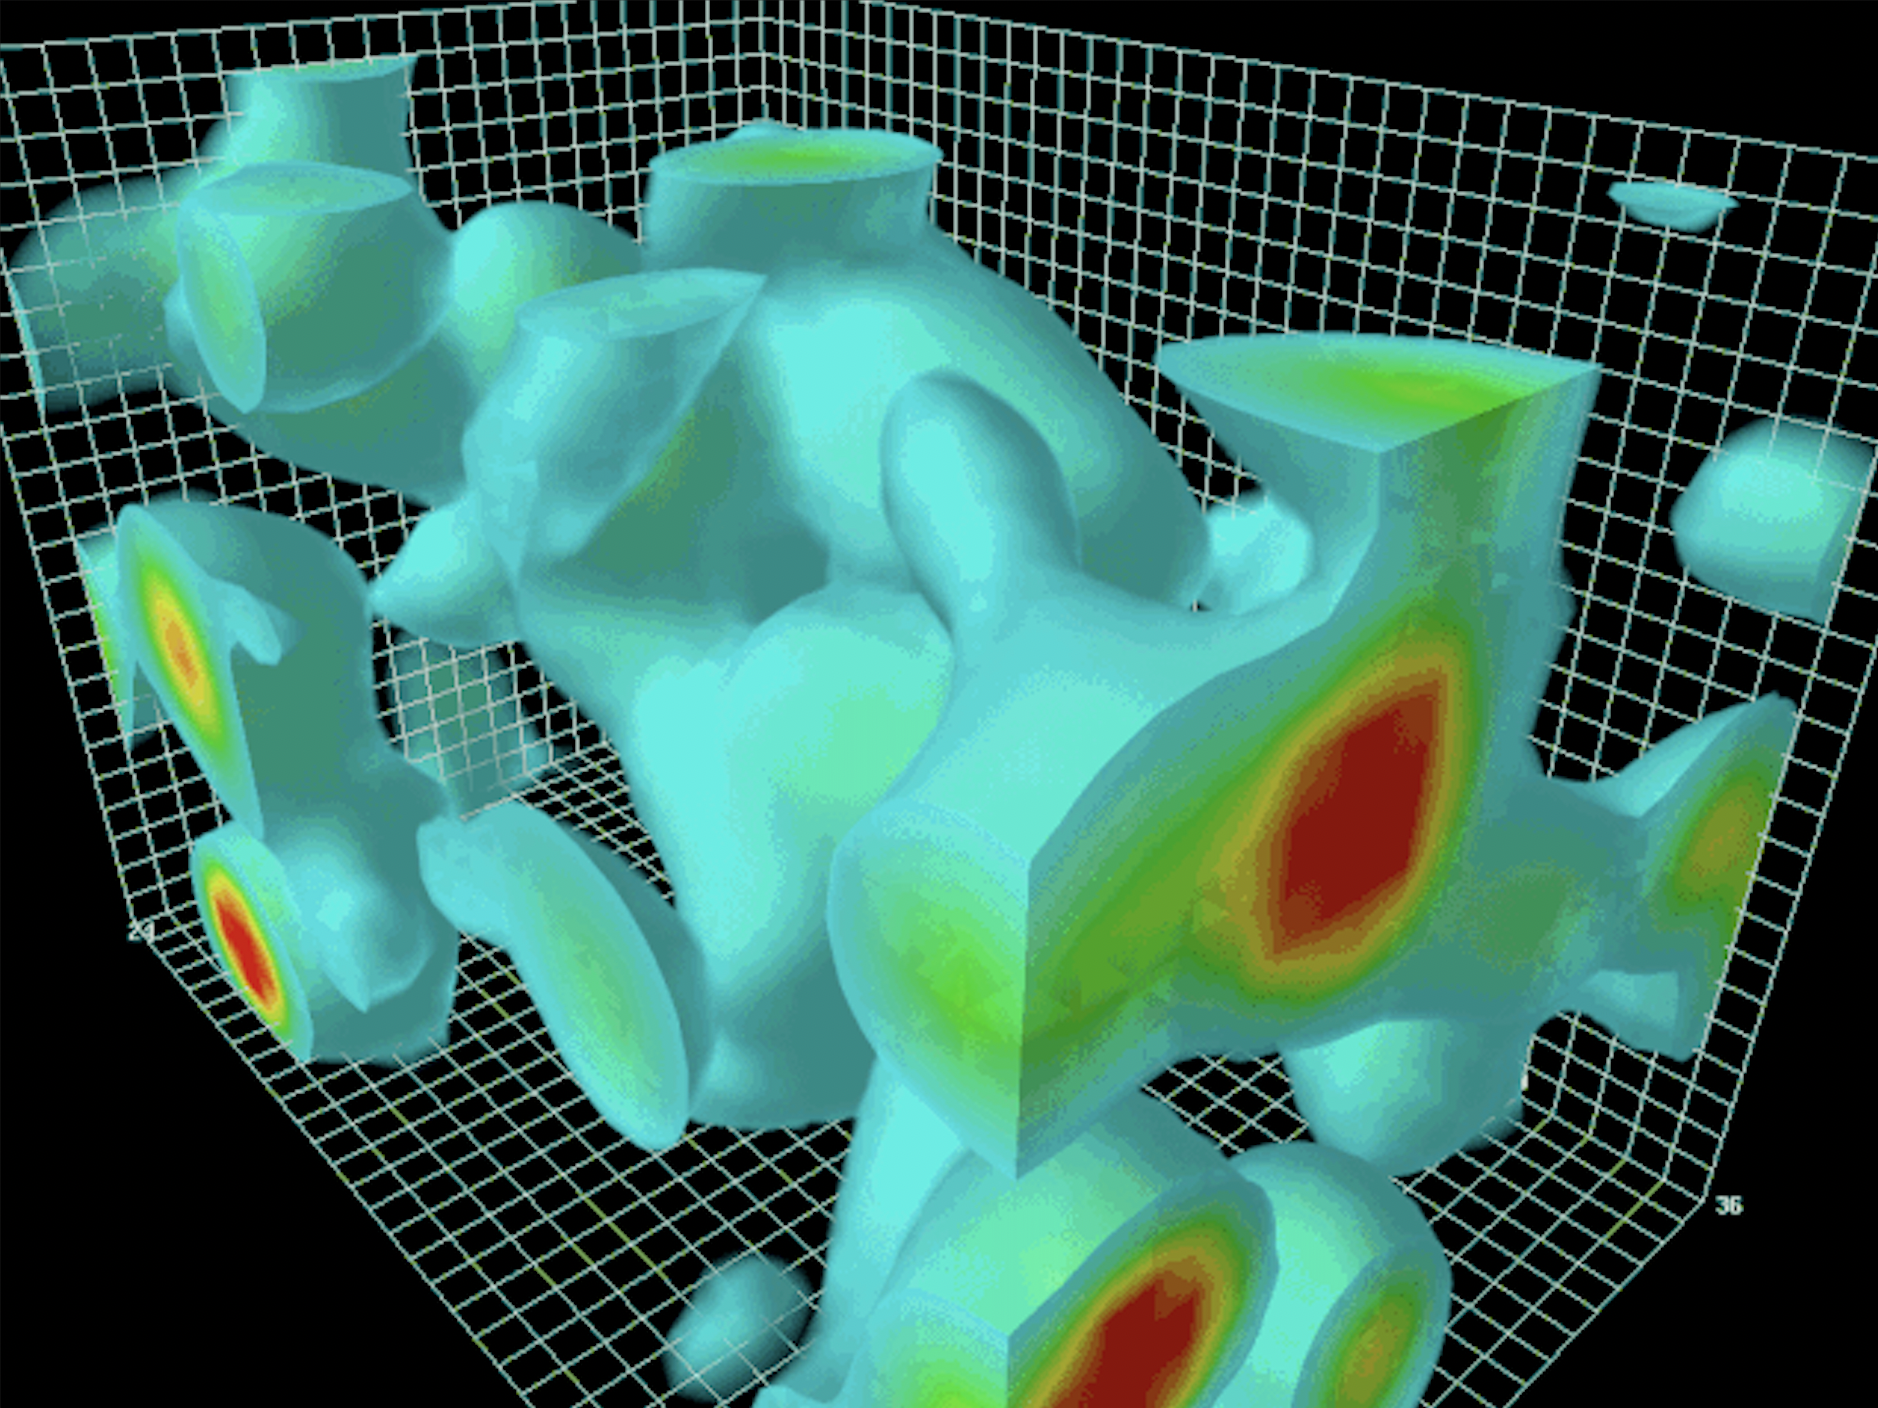
\includegraphics[width=0.5\linewidth]{fluc.png}
            \centering
            \caption{
                The volume of the box is 2.4 by 2.4 by 3.6 fm, big enough to hold a couple of protons. 
                Contrary to the concept of an empty vacuum, QCD induces chromo-electric and
                chromo-magnetic fields throughout space-time in its lowest energy state.
                [Center for the Subatomic Structure of Matter (CSSM) and Department of Physics, 
                University of Adelaide, 5005 Australia]\cite*{sim}}
            \label{Fluctuation}
        \end{figure}

    \section{The Casimir Effect}
        \begin{figure}
            \centering
            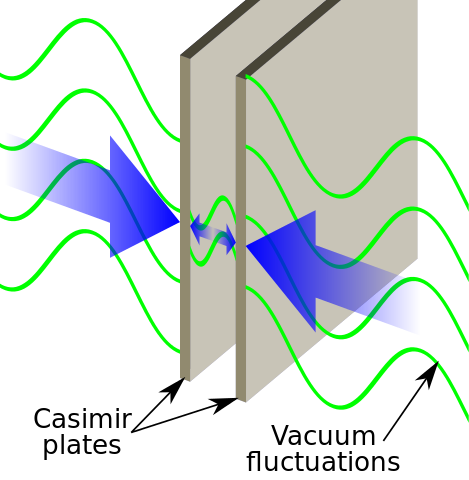
\includegraphics[width=0.5\linewidth]{plates.png}
            \caption{Two close parallel uncharged conducting plates. The green waves
            represent the quantum fluctuation in electromagnetic field.}
            \label{Plates}
        \end{figure}

        \paragraph{}
        The Casimir–Polder force. After a discussion with Niels Bohr, who suggested it had something to do with zero-point energy, Casimir alone formulated the theory predicting a force between neutral conducting plates in 1948, which is called the Casimir effect in the narrow sense.

        
        \paragraph{}
        The Casimir effect is force that arises from the quantum fluctuation of electromagnetic field in space, e.g., between two close parallel uncharged conducting plates, as in Figure~\ref{Plates}.
        To understand this effect consider those two close parallel conducting plates, they will trap 
        waves of fluctuating electromagnetic field as discussed in the previous section. But notice that 
        the longer-wavelength waves between the plates are vanished. Meaning that as the distance between
        the plates shrink the long wavelength waves cannot be fit. \cite*{casimir-sa} As result, the total energy exist between the 
        plates will be less, compared to elsewhere in the vacuum.

        \paragraph{}
        Due to this process the plates will attract to each other, as if they were connected to spring.
        This force can be given quantitatively by the formula \cite{byjus}
        \begin{align}
            F = \frac{\pi h c}{480} \frac{A}{L^4}
        \end{align}
        where $h$ is the Planck's constant, $A$ is the area of the plate, and $L$ is the spacing between the two plates. In specific, for two-one-meter square plates and with spacing between them, $10,000$ nanometer, they will exhibit a force order of $10^-7$ Newton.

    \section{Measuring the Casimir Effect}
        \paragraph{}
        Marcus Sparnaay, in 1958, conducted one of the first experimental tests in a delicate and challenging experiment with parallel plates, obtaining results not in contradiction with the Casimir theory but with significant experimental errors. A more accurate measurement of the Casimir effect was conducted by Steve K. Lamoreaux of Los Alamos National Laboratory and Umar Mohideen and Anushree Roy of California, Riverside. In practice, we use one flat plate and another plate that is a part of a sphere with a large radius to measure the Casimir effect because using two parallel plates would require accurate alignment to ensure they are parallel. Finally, in 2001, using microresonators, a group at the University of Padua succeeded in measuring the Casimir force between parallel plates.
    
    \section{Conclusion}
    In this article we leaned about the fascinating phenomenon that happens in vacuum, i.e., the quantum fluctuations of electromagnetic field. Moreover, we saw one of its consequences, the Casimir effect. In short, it is a force that appears between two uncharged conducting plates with very small spacing. This force tends to 
    push the plates into each other. This phenomenon has applications in the field nanotechnologies as well as affects in manufacturing the semiconductors' chips.


    \printbibliography
\end{document}